\let\negmedspace\undefined
\let\negthickspace\undefined
\documentclass[journal]{IEEEtran}
\usepackage[a4paper, margin=10mm, onecolumn]{geometry}
\usepackage{lmodern} % Ensure lmodern is loaded for pdflatex
\usepackage{tfrupee} % Include tfrupee package

\setlength{\headheight}{1cm} % Set the height of the header box
\setlength{\headsep}{0mm}  % Set the distance between the header box and the top of the text

\usepackage{gvv-book}
\usepackage{gvv}
\usepackage{cite}
\usepackage{amsmath,amssymb,amsfonts,amsthm}
\usepackage{algorithmic}
\usepackage{graphicx}
\usepackage{float}
\usepackage{textcomp}
\usepackage{xcolor}
\usepackage{txfonts}
\usepackage{listings}
\usepackage{enumitem}
\usepackage{mathtools}
\usepackage{gensymb}
\usepackage{comment}
\usepackage[breaklinks=true]{hyperref}
\usepackage{tkz-euclide} 
\usepackage{listings}
% \usepackage{gvv}                                        
\def\inputGnumericTable{}                                 
\usepackage[latin1]{inputenc}                                
\usepackage{color}                                            
\usepackage{array}                                            
\usepackage{longtable}                                       
\usepackage{calc}                                             
\usepackage{multirow}                                         
\usepackage{hhline}                                           
\usepackage{ifthen}                                           
\usepackage{lscape}
\usepackage{tikz}
\usetikzlibrary{patterns}

\begin{document}

\bibliographystyle{IEEEtran}
\vspace{3cm}

\title{9.2.32}
\author{EE25BTECH11064 - Yojit Manral}

\maketitle
% \maketitle
% \newpage
% \bigskip
{\let\newpage\relax\maketitle}
\renewcommand{\thefigure}{\theenumi}
\renewcommand{\thetable}{\theenumi}
\setlength{\intextsep}{10pt} % Space between text and float

\textbf{Question:}\\
Find the area of the region included between $y^2 = 9x$ and $y = x$.

\textbf{Solution:}\\
$\rightarrow$ The given conic can be expressed with parameters
\begin{align}
    \vec{V} = \myvec{0&0\\0&1}\text{, } \vec{u} = \myvec{-\frac{9}{2}\\0}\text{, } f = 0
\end{align}
$\rightarrow$ The given line can be expressed with the parameters
\begin{align}
    \vec{h} = \myvec{0\\0}\text{, } \vec{m} = \myvec{1\\1}
\end{align}
$\rightarrow$ The point of intersection of the line
\begin{align}
    \vec{L} \equiv \vec{x} = \vec{h} + \kappa\vec{m}
\end{align}
\hspace{0.3cm} with a general conic
\begin{align}
    g\brak{\vec{x}} = \vec{x}^T\vec{V}\vec{x} + 2\vec{u}^T\vec{x} + f = 0
\end{align}
\hspace{0.3cm} can be given by
\begin{align}
    \vec{x_i} = \vec{h} + \kappa_i\vec{m}
\end{align}
\hspace{0.3cm} where
\begin{align}
    \kappa_i = \frac{1}{\vec{m}^T\vec{V}\vec{m}}\brak{-\vec{m}^T\brak{\vec{V}\vec{h}+\vec{u}}\pm \sqrt{\brak{\vec{m}^T\brak{\vec{V}\vec{h}+\vec{u}}}^2-g\brak{\vec{h}}\brak{\vec{m}^T\vec{V}\vec{m}}}}
\end{align}
$\rightarrow$ Substituting the parameters from (1), (2) in (6), we get
\begin{align}
    \vec{x_1} = \myvec{0\\0}\text{, } \vec{x_2} = \myvec{9\\9}
\end{align}
$\rightarrow$ From the figure, the area bounded by the conic $y^2 = 9x$ and the line $y = x$ is given by
\begin{align}
    \int_{0}^{9}\brak{3\sqrt{x} - x}dx &= \left[2(x)^{3/2} - \frac{x^2}{2}\right]_{0}^{9} = \frac{27}{2}\hspace{0.2cm}units
\end{align}
\begin{figure}[h!]
   \centering
   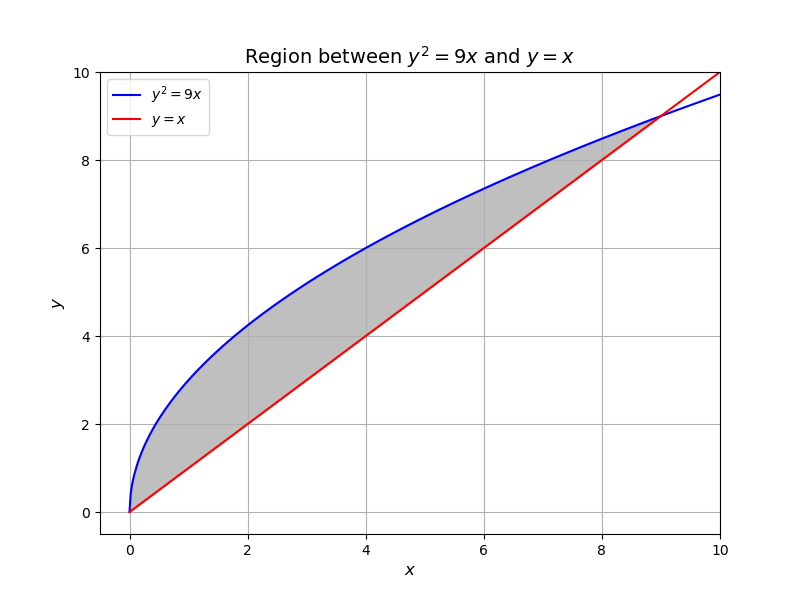
\includegraphics[width=0.7\linewidth]{figs/01.png}
   \caption{Plot of $y^2 = 9x$ and $y = x$}
   \label{Plot_1}
\end{figure}
\end{document}
